% !TEX encoding = UTF-8 Unicode

\section{Descrição Atualizada da Linguagem em Wirth}

\lstinputlisting[frame=single,numbers=left,breaklines=true,basicstyle=\ttfamily\scriptsize]{files/WIRTH_atualizado.txt}

\section{Lista de Autômatos do APE}

\begin{itemize}

	\item ATOMO-COND:
	\begin{figure}[H]
		\centering 
		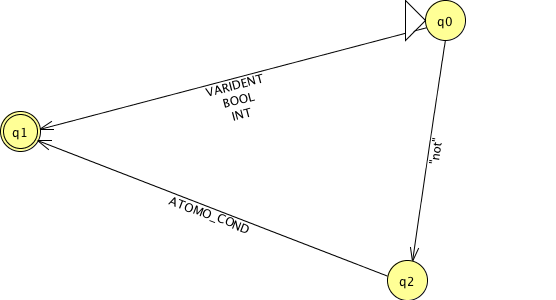
\includegraphics[width=0.8\textwidth]{images/submaquinas/ATOMO-COND.png}  
		\caption{Autômato ATOMO-COND}
	\end{figure}
	
	\item ATOMO:
	\begin{figure}[H]
		\centering 
		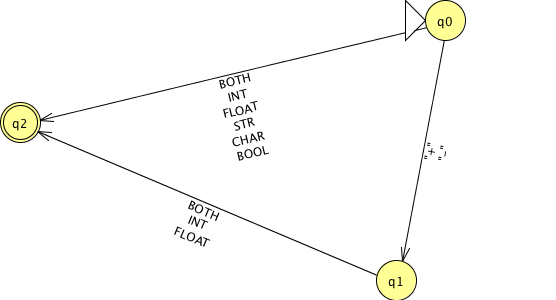
\includegraphics[width=0.8\textwidth]{images/submaquinas/ATOMO.png}  
		\caption{Autômato ATOMO}
	\end{figure}
	
	\item BOTH:
	\begin{figure}[H]
		\centering 
		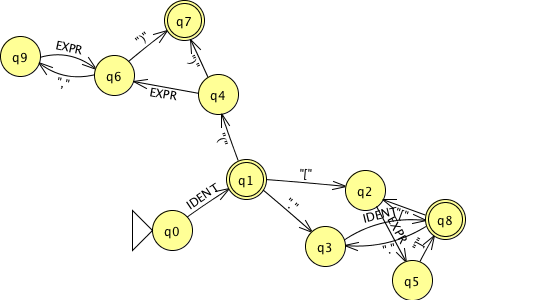
\includegraphics[width=0.8\textwidth]{images/submaquinas/BOTH.png}  
		\caption{Autômato BOTH}
	\end{figure}
	
	\item COND-TERM:
	\begin{figure}[H]
		\centering 
		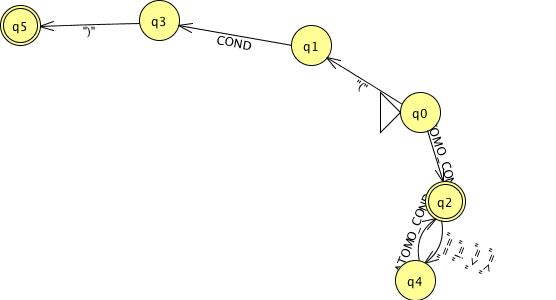
\includegraphics[width=0.8\textwidth]{images/submaquinas/COND-TERM.png}  
		\caption{Autômato COND-TERM}
	\end{figure}
	
	\item COND:
	\begin{figure}[H]
		\centering 
		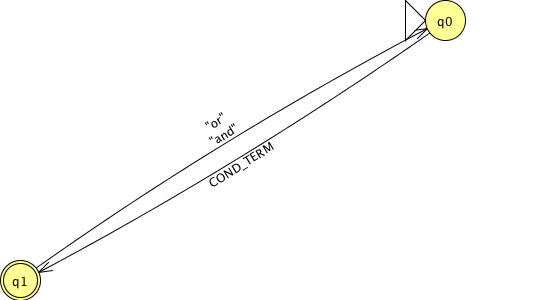
\includegraphics[width=0.8\textwidth]{images/submaquinas/COND.png}  
		\caption{Autômato COND}
	\end{figure}
	
	\item DECLS-GLOBAIS:
	\begin{figure}[H]
		\centering 
		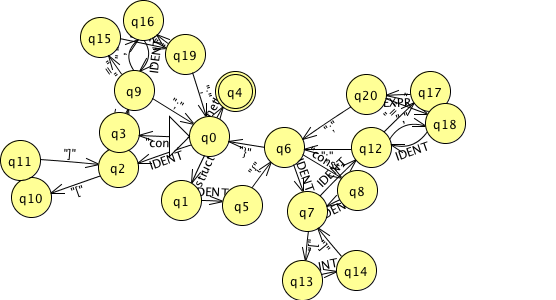
\includegraphics[width=0.8\textwidth]{images/submaquinas/DECLS-GLOBAIS.png}  
		\caption{Autômato DECLS-GLOBAIS}
	\end{figure}
	
	\item DEF-MAIN:
	\begin{figure}[H]
		\centering 
		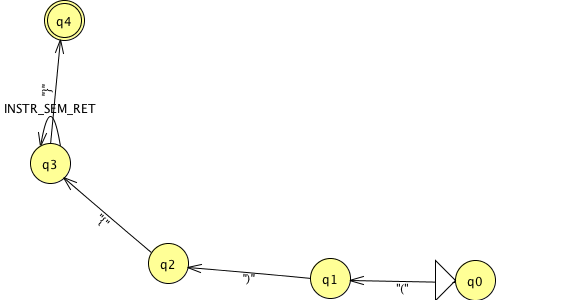
\includegraphics[width=0.8\textwidth]{images/submaquinas/DEF-MAIN.png}  
		\caption{Autômato DEF-MAIN}
	\end{figure}
	
	\item DEF-PROCS-FUNCS:
	\begin{figure}[H]
		\centering 
		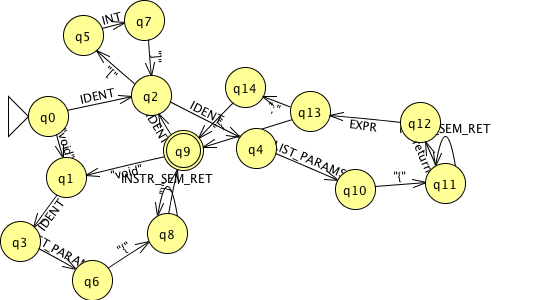
\includegraphics[width=0.8\textwidth]{images/submaquinas/DEF-PROCS-FUNCS.png}  
		\caption{Autômato DEF-PROCS-FUNCS}
	\end{figure}
	
	\item EXPR:
	\begin{figure}[H]
		\centering 
		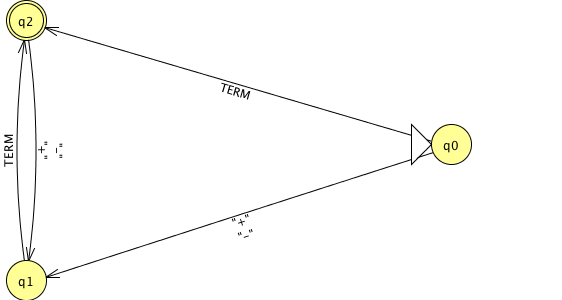
\includegraphics[width=0.8\textwidth]{images/submaquinas/EXPR.png}  
		\caption{Autômato EXPR}
	\end{figure}
	
	\item FUNCTION-CALL:
	\begin{figure}[H]
		\centering 
		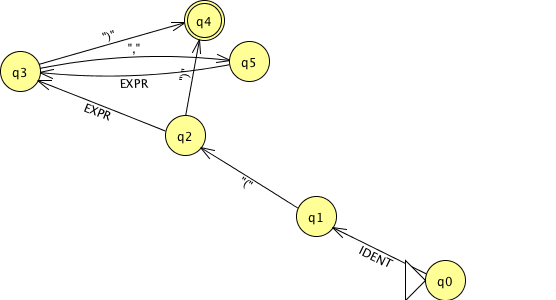
\includegraphics[width=0.8\textwidth]{images/submaquinas/FUNCTION-CALL.png}  
		\caption{Autômato FUNCTION-CALL}
	\end{figure}
	
	\item IMPORTS:
	\begin{figure}[H]
		\centering 
		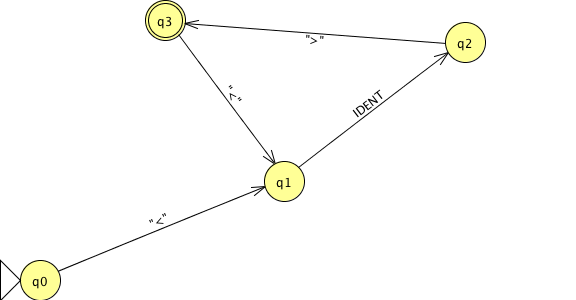
\includegraphics[width=0.8\textwidth]{images/submaquinas/IMPORTS.png}  
		\caption{Autômato IMPORTS}
	\end{figure}
	
	\item INSTR-SEM-RET:
	\begin{figure}[H]
		\centering 
		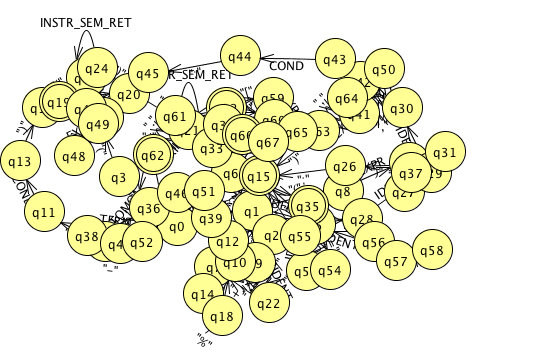
\includegraphics[width=1.0\textwidth]{images/submaquinas/INSTR-SEM-RET.png}  
		\caption{Autômato INSTR-SEM-RET}
	\end{figure}
	
	\item LIST-PARAMS:
	\begin{figure}[H]
		\centering 
		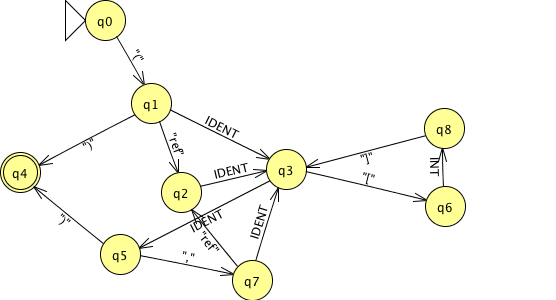
\includegraphics[width=0.8\textwidth]{images/submaquinas/LIST-PARAMS.png}  
		\caption{Autômato LIST-PARAMS}
	\end{figure}
	
	\item OPER-ATRIB:
	\begin{figure}[H]
		\centering 
		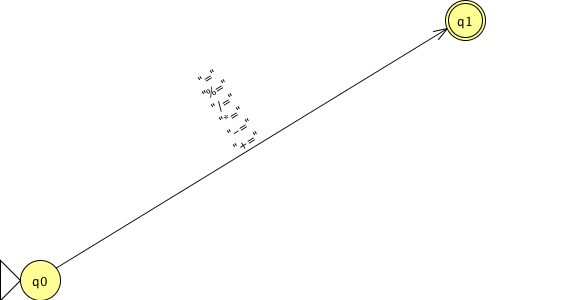
\includegraphics[width=0.8\textwidth]{images/submaquinas/OPER-ATRIB.png}  
		\caption{Autômato OPER-ATRIB}
	\end{figure}
	
	\item PROGRAM:
	\begin{figure}[H]
		\centering 
		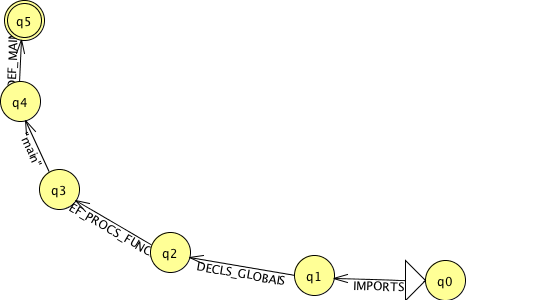
\includegraphics[width=0.8\textwidth]{images/submaquinas/PROGRAM.png}  
		\caption{Autômato PROGRAM}
	\end{figure}
	
	\item TERM:
	\begin{figure}[H]
		\centering 
		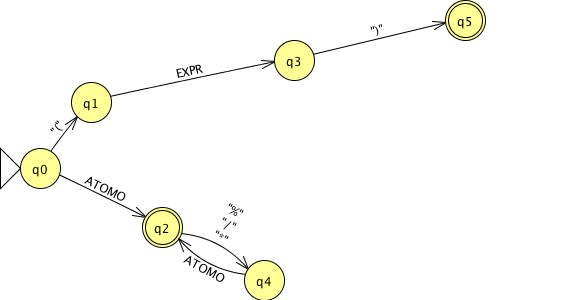
\includegraphics[width=0.8\textwidth]{images/submaquinas/TERM.png}  
		\caption{Autômato TERM}
	\end{figure}
	
	\item VARIDENT:
	\begin{figure}[H]
		\centering 
		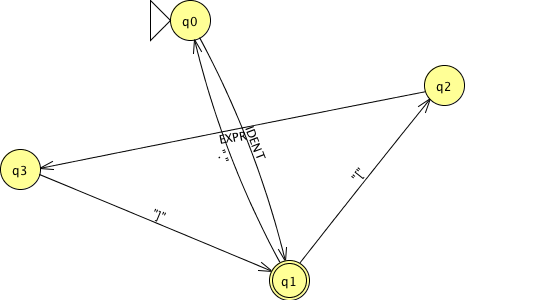
\includegraphics[width=0.8\textwidth]{images/submaquinas/VARIDENT.png}  
		\caption{Autômato VARIDENT}
	\end{figure}

\end{itemize}
